\subsection{\label{subsec:FZV3}Frage 3}
\textbf{\textit{Erläutern Sie den experimentellen Aufbau und die Funktionsweise eines Dunkelfeldmikroskops
in Transmission. Fertigen Sie dazu eine Skizze mit dem Strahlengang an. 
Wo muss die DF-Maske genau platziert werden?}} \\
$\rightarrow$Die Dunkelfeldspektroskopie in Transmission ist eine Technik, die es ermöglicht, das Streulicht von Objekten zu analysieren, 
während das direkt durchgelassene Licht blockiert wird. Hierzu benötigt man eine Lichtquelle dessen Lichtstrahlen 
gegebenenfalls mit einem Polarisator und einen Kollimator, polarisiert und parallelisiert werden.
Eine Dunkelfeldmaske (inverse Lochblende), die den Unterschied zur Absorptionsspektroskopie bildet, lässt nur 
die Ränder des Erregerlichtkegels passieren. 
Dieses Licht wird von einem Objektiv hoher numerischer Apertur oder einem Kondensor auf die Probe geleitet. 
Das Beleuchtungsprofil wird dabei so eingestellt, dass das Objektiv hinter der Probe hiervon 
nicht bestrahlt wird. Vernachlässigt man Störeffekte aus anderen Quellen, erreicht den Detektor 
(hinter Analyse-Objektiv und Sammellinse) folglich nur
Streulicht der Probe, was eine gute Analyse ermöglicht.
Eine aus der Versuchsanleitung \cite{Anleitung} entnommene Skizze eines Dunkelfeldspektroskops 
ist in Abb.~\ref{fig:aufbau} dargestellt. 
\begin{figure}[h!]
    \centering
    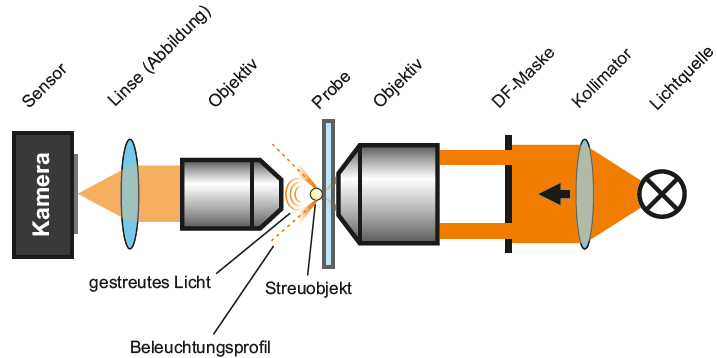
\includegraphics[width=0.8\textwidth]{Dunkel.png}
    \caption{\label{fig:aufbau}Skizze des Strahlengangs eines Dunkelfeldmikroskops in Transmission.
    Die Bestandteile sind beschriftet und deren Aufgabe ist im Haupttext beschrieben.}
\end{figure}\FloatBarrier
Die DF-Maske sollte möglichst nahe an das erste Objektiv gebracht werden, um die Divergenz des 
transmittierten Lichtes gering zu halten. Dadurch wird sichergestellt, dass das Analyse-Objekt
kein Licht der Quelle erreicht und zusätzlich wird der Übergang zwischen Dunkelfeld- und 
Absorptionsspektroskopie (entfernen der Maske) erleichtert, da keine neue Justage notwendig ist. 

